\chapter{Introduction}

%\section{Household robots in general}
More and more robots appear in everyday life. Automatic vacuum cleaners and floor washers are getting widespread, as the technology is becoming cheaper and better. The vacuum cleaners have matured to a level, where they are been considered for saving man-hours in the elderly care sector.\\\\
\noindent
Outside the walls of our homes lays the next weekly hurdle: mowing the lawn. A known way to handle this, is to pay the neighbour's teenager to do it. Unfortunately they grow up and move out, leaving the lawns in the residential neighbourhoods behind.\\\\
\noindent
Luckily engineers have stepped in, and provided a more long-term solution: robotic lawn mowers.

\section{Robotic lawn mowers}
Several manufacturers of electrical gardening machines have started selling robotic lawn mowers in the recent years. In general they use one of two strategies when cutting the lawn:
\begin{itemize}
	\item Random direction mowers
	\item Parallel line mowers
\end{itemize}

\noindent
Mowers using the random direction strategy will drive in a straight line until a guard wire or an obstacle is detected. They will then turn in a random direction, and continue. See \figref{fig:randomcut}

\begin{figure}[H]
\centering
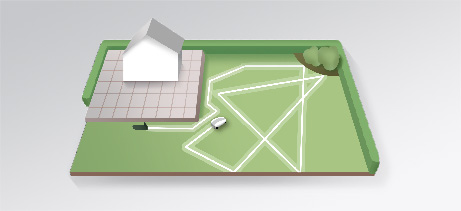
\includegraphics[scale=0.8]{figures/noLogiCut.jpg} 
\label{fig:randomcut}
\caption{Random cut system [source:Bosch]} 
\end{figure}

\noindent
When the battery is nearly discharged, the mower will follow the guard wire back to the base station for recharging.\\\\
\noindent
Parallel line mowers use a more intelligent control algorithm to optimize the mowing. After an initial learning run, following the guard wire around the lawn to be mowed, it will map the lawn, and cut in parallel lines, see \figref{fig:logicut}. The advantage of this strategy efficiency, as the lawn mower will not run over the same spots more than once. According to Bosch, a given lawn can be mowed up to 30\% faster with their Logicut system.
%% TODO: Insert source
 

\begin{figure}[H]
\centering
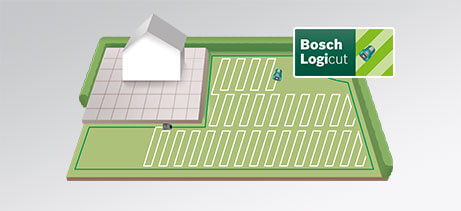
\includegraphics[scale=0.8]{figures/logicut.jpg} 
\label{fig:logicut}
\caption{Bosch Logicut system [source:Bosch]} 
\end{figure}

\noindent
Common for both systems is the guard wire, which has to be placed around the lawn and anywhere the lawn mower is not allowed to go, like flower beds, swimming pools, etc. \\\\
\noindent
This brings us to the problem with existing products.

\section{Problems with existing robotic lawn mowers}
All commercially available robotic lawn mowers requires a guard wire placed around the lawn. This can either be placed at the surface, and be held in place by pegs, or dug down below the surface. The guard wire must be routed around flower beds, etc. as well, see \figref{fig:robomow}

 
\begin{figure}[H]
\centering
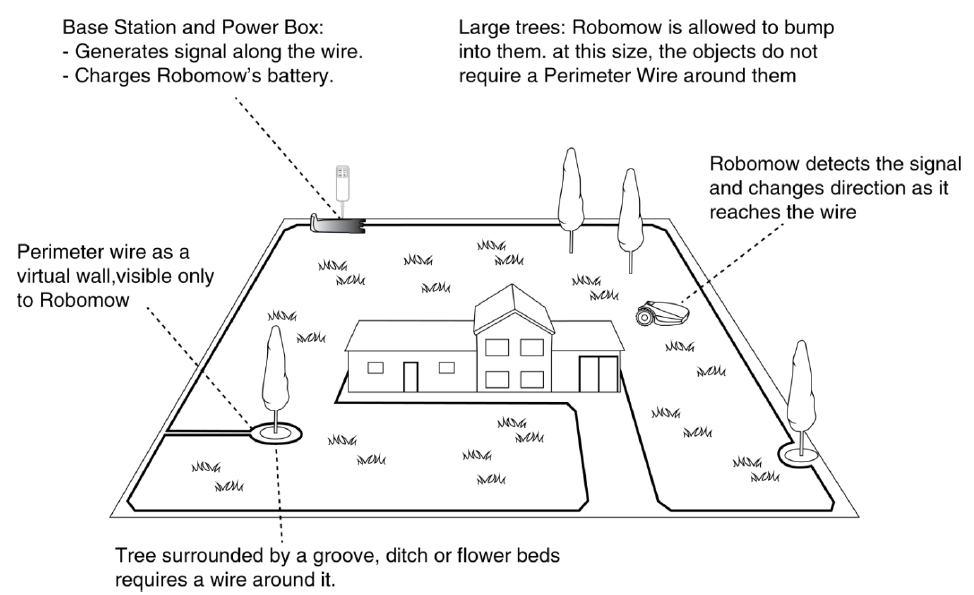
\includegraphics[scale=0.6]{figures/robomow.png} 
\label{fig:robomow}
\caption{Guard wire installation [source:Robomow]} 
\end{figure}
\noindent

The use of the guard wire for guiding the mower back to the charging station presents another potential problem: in a garden with many restricted areas, the guard wire could get very long. This could therefore make the journey home long, compared to a more direct route. This again uses more battery power, that instead could have been used for actually mowing the lawn.\\\\
\noindent
This will be the motivation for the project: to avoid the work routing a wire around the garden, and as a bonus get more work done on a battery charge, by not wasting power following the wire home.\\\\
\noindent
Then, the question is: What other solutions could be use to get the lawn mower to go where it has to go? \\
One first step could be to keep track of where it is in real-time.
%-- Section : GoT introductory presentation --%
\section{The Games on Track (GoT) system}
We were provided with the \emph{Games on Track GT-Position} system as a start to be able to determine the lawn mower's position in space. 
% Add reference to GoT description

\begin{figure}[H]
\centering
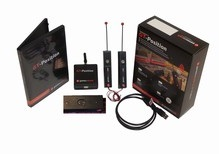
\includegraphics[scale=1.1]{figures/gotSystem.jpg} 
\label{fig:gotsystem}
\caption{Games on Track GT-Position package [source:Games\ on\ Track]} 
\end{figure}
\noindent

\noindent
It is composed of four different parts both hardware and software :
%% TODO : Add reference to http://www.gamesontrack.co.uk/pages/webside.asp?articleGuid=64556
\begin{itemize}
	\item A tracked module, which emits ultra-sound waves. It should be placed on the lawn mower itself while taking care, that the emitting cell is not obstructed by anything.
	\item Beacons or receivers, placed around the area the lawn mower will move in. Depending on the terrain, anywhere from 2 \todo{--Resolved-- is two enough? Answer: It is according to the GoT site (see reference in LaTeX comments)} to more than 20 of these can be used: the more is placed, the more accuracy can be obtained to fight against any ambient noise.
	\item The central system, which calculates the distance of the tracked module to each beacon, and transmits it to the computer via USB in regular intervals.
	\item The GoT software aggregates the received positions throughout time, and can be used to draw a map of the terrain (the lawn), and to determine the absolute position of the tracked module.
\end{itemize}

GoT was originally designed for train modelling, but it is easily adaptable for any use of position tracking and seems a good choice, at first, for our autonomous lawn mower.
But, why not use a satellite based positioning system ?

%-- Section : Satellite vs GoT --%
\section{Satellite based positioning systems vs GoT}
\todo{Wrong reasons for GPS vs GoT, elaborated below}
The reasons why satellite positioning system won't be used in our project are mainly related to accuracy over price ratios and to energy consumption.\todo{--To be reviewed again-- GPS uses very little power -> depending on the accuracy needed...}

\noindent
Indeed, these kinds of system like GPS or GLONASS would require a dedicated chip to put on the final system. The problem then would be the lack of precision. Although, there are some cheap standard GPS chips (around USD 10), these only reach around 1 meter of precision in the most ideal situations. % ref : www.gps.gov
On the other hand, the best GPS chips can achieve precisions up to a few millimeters when combined with different augmentation systems (algortihms for instance), but they end up being highly expensive (usually thousands of dollars). They are not generally intended for public use.
\todo{--To be reviewed again-- Only applies to cheap solutions, differential GPS can go to mm level, but is extremely expensive. This is what we are trying to replace with GoT, as it is a lot cheaper than diff-GPS} \\\\
%% TODO : Add reference to "A Review of GLONASS" Miller, 2000 & http://www.gps.gov/systems/gps/performance/accuracy/ 
\noindent
Moreover, if we add up the slow bit rates satellites can achieve, the signal amplifiers on the receiver, plus all the position calculations and possible augmentation systems, the total energy consumption would quickly rise,\todo{--To be reviewed again-- nope, it's just a radio receiver, uses almost no power} thus reducing the lawn mower autonomy, which is not desirable.\\
Indeed, the design of a product has no real value if no one is interested in using it. This is why choices made during this project have to be made in accordance with the final user's expectations.\\\\
\section{Potential consumer expectations}
Usually, we can think of a few priorities consumers will have when buying a product, whatever it is, and some more specific to technical products.\\
\noindent
Here for instance, the autonomy of the vehicle (both in energy and for the navigation), and the overall cost should be considered. The GoT system itself has a cost (USD 606.00 for a basic package) beyond anything a normal customer would probably pay for a lawn mower. But despite that, it appears, at first, to be a good solution for us in terms of accuracy and energy consumption compared to GPS-like systems which are even more expensive for the same accuracy. \todo{--Resolved-- insert price approximation here - not so true actually} \\\\
\noindent
These are the types of preliminary considerations that will influence this design process for an autonomous lawn mower.